\chapter{\label{ch:ch01}ГЛАВА 1. Обзор Godot} % Нужно сделать главу в содержании заглавными буквами

\section{\label{sec:ch01/sec01}Раздел 1. Возможности Godot}

\subsection{\label{subsec:ch01/sec01/sub01}Описание движка}

Godot - это универсальный и простой в освоении игровой движок, который позволяет создавать как 2D, так и 3D игры. Он обладает широким спектром возможностей, делающих его привлекательным выбором как для начинающих, так и для опытных разработчиков.

\subsection{\label{subsec:ch01/sec01/sub02}2D и 3D возможности Godot}

\textbf{2D:}

\begin{itemize}
    \item Создание 2D персонажей, окружения и интерфейсов.
    \item Плавная анимация с использованием спрайтов, скелетной анимации и tween-инструментов.
    \item Физика 2D с реалистичными столкновениями и взаимодействиями.
    \item Tilemaps для создания уровней с повторяющимися элементами.
    \item Камеры с эффектами параллакса, приближения и тряски.
    \item Частицы для создания визуальных эффектов, таких как взрывы, дождь и огонь.
\end{itemize}

\textbf{3D:}

\begin{itemize}
    \item 3D моделирование и импорт из популярных форматов (OBJ, FBX и т.д.).
    \item PBR-шейдеры для реалистичного освещения и материалов.
    \item Физика 3D с Bullet Physics Engine.
    \item Анимация персонажей с использованием скелетной анимации.
    \item Редактор для создания 3D ландшафтов.
    \item Эффекты пост-обработки для лучшего визуального качества игры.
\end{itemize}


\subsection{\label{subsec:ch01/sec01/sub02}Система, основанная на "нодах"}

Godot использует уникальную node-based систему для организации игровых объектов и их взаимодействия. Это позволяет разработчикам легко создавать сложные сцены и управлять объектами через иерархию узлов. У каждого "нода" есть свои параметры и "дети" которые наследуют некоторые характеристики "родителя", что позволяет создавать различные взаимодействия между объектами чуть легче, чем в других движках.

\section{\label{sec:ch01/sec02}Раздел 2: много уровневые списки}

\subsection{\label{subsec:ch01/sec02/sub01}Подраздел 1: пример нумерованного списка}

Пример вложенного нумерованного списка:
\begin{enumerate}
\item Первый элемент:
\begin{enumerate}
\item Первый элемент первого элемента;
\item Второй элемент первого элемента;
\end{enumerate}
\item Второй элемент:
\begin{enumerate}
\item Первый элемент второго элемента;
\item Второй элемент второго элемента.
\end{enumerate}
\end{enumerate}

\subsection{\label{subsec:ch01/sec02/sub02}Подраздел 2: пример маркерованного списка}

Пример вложенного маркерованного списка:
\begin{itemize}
\item первый элемент:
\begin{itemize}
\item первый элемент первого элемента;
\item второй элемент первого элемента;
\end{itemize}
\item Второй элемент:
\begin{itemize}
\item первый элемент второго элемента;
\item второй элемент второго элемента.
\end{itemize}
\end{itemize}

Пример ссылки на рисунок в документе~\ref{fig:example01}.
\begin{figure}[h]
    \centering
    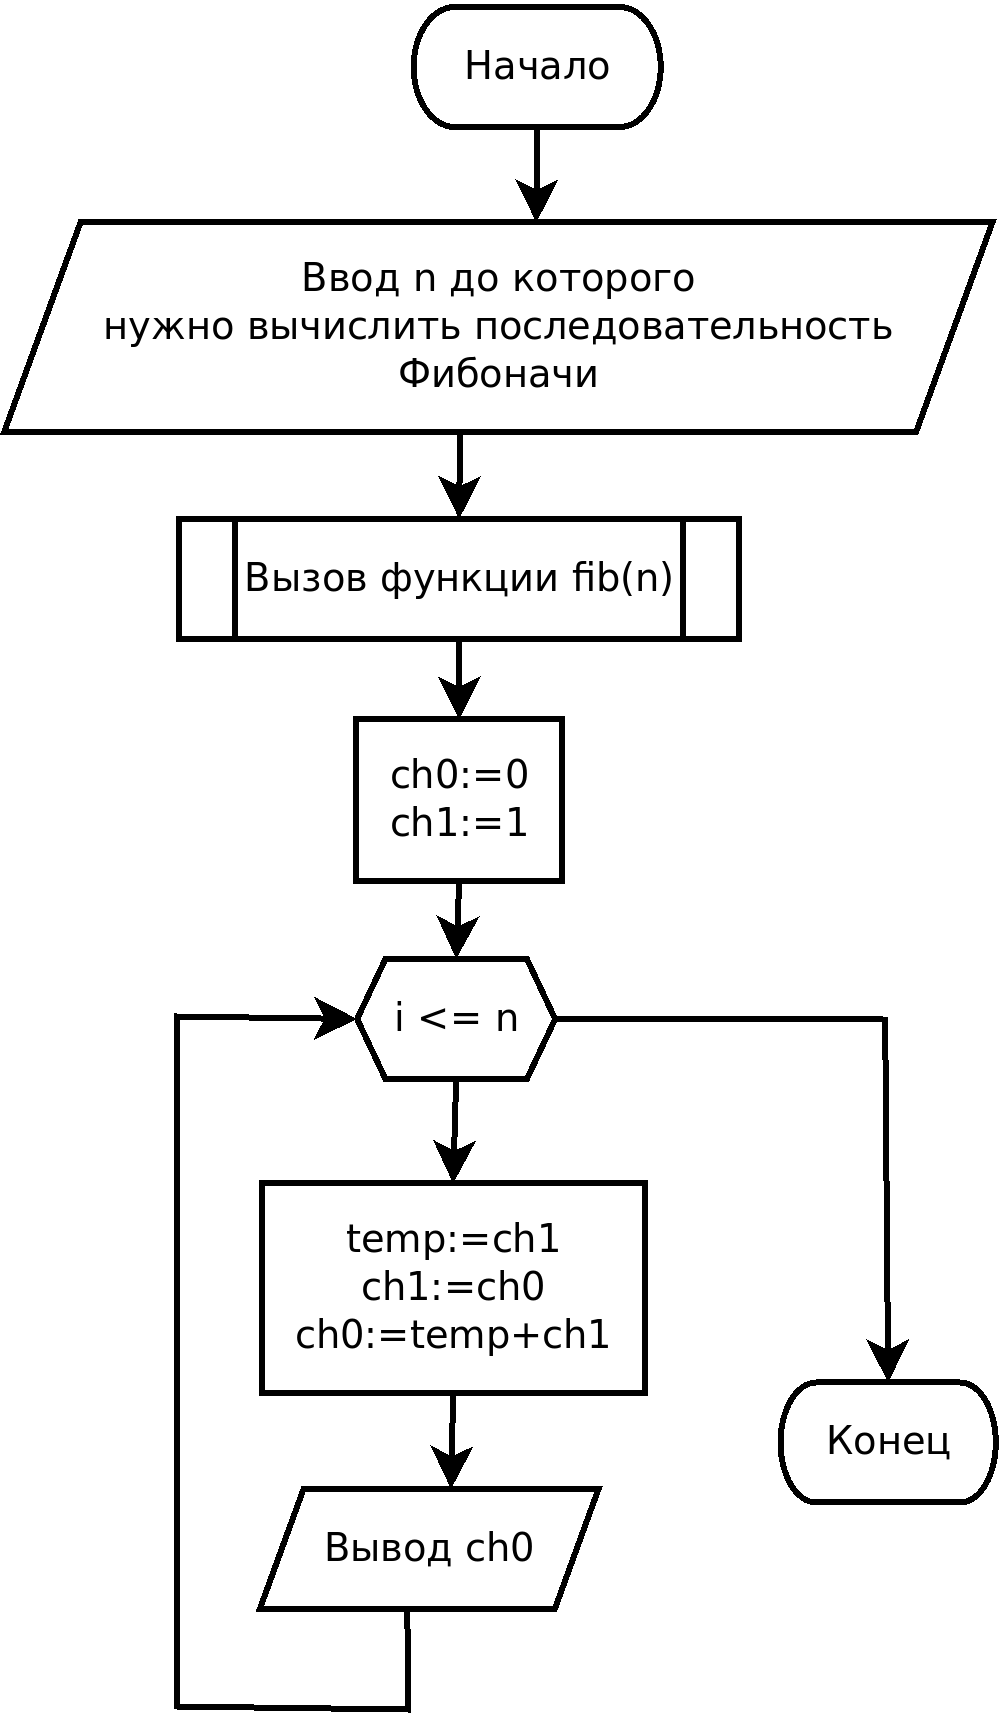
\includegraphics[width=0.5\textwidth]{./images/fibonacci.png}
    \caption{\centering\label{fig:example01}Пример рисунка в формате PNG.}
\end{figure}

Пример ссылки на рисунок в документе~\ref{fig:example02}.
\begin{figure}[h]
    \centering
    \includesvg[width=0.5\textwidth]{./images/fibonacci.svg}
    \caption{\centering\label{fig:example02}Пример рисунка в формате SVG.}
\end{figure}

Пример ссылки на таблицу в документе~\ref{tab:example01}.
\begin{table}[H]
\caption{\centering\label{tab:example01}Системные требования}
\begin{tabular}{|p{3 cm}|p{3 cm}|p{3 cm}|p{5 cm}|}
\hline
Минимальные требования & 1 & 2 & 3 \\ \hline
Версия операционной системы & 1 & 2 & 3 \\ \hline
Процессор & 1 & 2 & 3 \\ \hline
Графический API & 1 & 2 & 3 \\ \hline
\end{tabular}
\end{table}

Пример ссылки на таблицу в документе~\ref{tab:example02}.
\begin{table}[H]
\caption{\centering\label{tab:example02}Системные требования}
\begin{tabular}{|p{3 cm}|p{3 cm}|p{3 cm}|p{5 cm}|}
\hline
Минимальные требования & 1 & 2 & 3 \\ \hline
Версия операционной системы & 1 & 2 & 3 \\ \hline
Процессор & 1 & 2 & 3 \\ \hline
Графический API & 1 & 2 & 3 \\ \hline
\end{tabular}
\end{table}

Пример использования minted для оформления кода и ссылка на этот код~\ref{code:fibonacci}.
\begin{code}
\captionof{listing}{\centering\label{code:fibonacci}Пример программы вычисления n-ой последовательности Фибоначчи}
\vspace{-\baselineskip}\inputminted{python}{src/fibonacci.py}
\end{code}

Пример использования minted для оформления кода и ссылка на этот код~\ref{code:example02}.
\begin{code}
\captionof{listing}{\centering\label{code:example02}Сложение двух массивов параллельно десятью потоками (пример из https://ru.wikipedia.org/wiki/OpenMP)}
\vspace{-\baselineskip}\begin{minted}{C}
#include <stdio.h>
#include <omp.h>
#define N 100

int main(int argc, char *argv[]) {
  double a[N], b[N], c[N];
  int i;
  omp_set_dynamic(0); // запретить библиотеке openmp менять число потоков во время исполнения
  omp_set_num_threads(10); // установить число потоков в 10
  // инициализируем массивы
  for (i = 0; i < N; i++) {
      a[i] = i * 1.0;
      b[i] = i * 2.0;
  }
  // вычисляем сумму массивов
#pragma omp parallel for shared(a, b, c) private(i)
   for (i = 0; i < N; i++)
     c[i] = a[i] + b[i];

  printf ("%f\n", c[10]);
  return 0;
}
\end{minted}
\end{code}
